%\documentclass[handout]{beamer}
\documentclass{beamer}
\usepackage{amsmath}
\usepackage{stdpresent}
\usepackage{todonotes}
%\usepackage[margin=1in]{geometry}
\usepackage{tikz}
\usepackage{booktabs}
\usetikzlibrary{intersections,positioning}
\usetikzlibrary{matrix, calc}
\newcommand*{\hnode}[1]{\node[outer sep=0pt,anchor=base] (#1) {#1};} 
\usepackage[absolute,overlay]{textpos}
\usetikzlibrary{bayesnet}
\usepackage{tcolorbox}
\usepackage[round]{natbib}
\usepackage{multirow}
\usepackage{subfig}
\usepackage{color}
\newcommand{\ack}[1]{\let\thefootnote\relax\footnote{\textcolor{gray}{#1}}}
\usepackage[tikz]{bclogo}
% Custom macros
\newcommand{\angbrack}[1]{\ensuremath{\langle #1 \rangle}}
\newcommand{\cc}[1]{$\dagger$\marginpar{\fbox{\parbox{19mm}{\scriptsize #1}}}}
\interfootnotelinepenalty=10000
\newcommand{\reftab}[1]{Table~\ref{tab:#1}}
\newcommand{\refeq}[1]{Equation~\ref{eq:#1}}
\newcommand{\reffig}[1]{Figure~\ref{fig:#1}}
\newcommand{\refalg}[1]{Algorithm~\ref{alg:#1}}
\newcommand{\refsec}[1]{Section~\ref{sec:#1}}
\newcommand{\dx}{\ensuremath{{d_{\texttt{x}}}}}
\newcommand{\dhidden}{\ensuremath{{d_{\texttt{h}}}}}
%\newcommand{\dw}{\ensuremath{{d_{\texttt{\omega}}}}}
\newcommand{\ds}{\ensuremath{{d_{\texttt{s}}}}}
\newcommand{\vx}{\ensuremath{{v_{\texttt{x}}}}}
\newcommand{\vy}{\ensuremath{{v_{\texttt{y}}}}}
\newcommand{\txt}[1]{{\ensuremath{\text{#1}}}}
\DeclareMathOperator{\KL}{KL}
\DeclareMathOperator{\R}{R}
\DeclareMathOperator{\vMF}{vMF}
\DeclareMathOperator{\diag}{diag}
\DeclareMathOperator{\Cat}{Cat}
\DeclareMathOperator{\Ray}{Rayleigh}
\DeclareMathOperator{\Bern}{Bern}
\DeclareMathOperator{\Beta}{Beta}
\DeclareMathOperator{\ELBO}{ELBO}
\DeclareMathOperator{\encode}{encode}
\DeclareMathOperator{\MLP}{MLP}
\DeclareMathOperator{\softmax}{softmax}
\DeclareMathOperator{\softplus}{softplus}
\DeclareMathOperator{\sigmoid}{sigmoid}
\DeclareMathOperator{\onehot}{one-hot}
\DeclareMathOperator{\emb}{emb}
\DeclareMathOperator{\rnn}{rnn}
\DeclareMathOperator{\birnn}{birnn}
\DeclareMathOperator{\loc}{location}
\DeclareMathOperator{\scale}{scale}
\DeclareMathOperator{\att}{attention}
\DeclareMathOperator{\affine}{affine}
\DeclareMathOperator{\concat}{concat}
\DeclareMathOperator{\compose}{compose}
\DeclareMathOperator{\avg}{avg}
\DeclareMathOperator{\maxpool}{maxpool}
\DeclareMathOperator{\mlp}{mlp}
\DeclareMathOperator{\layer}{layer}
\DeclareMathOperator{\gauss}{gauss}
\DeclareMathOperator{\spherical}{vmf}
\DeclareMathOperator{\relu}{ReLu}
\DeclareMathOperator{\css}{css}
\newcommand{\Lx}{\texttt{L1}\xspace}
\newcommand{\Ly}{\texttt{L2}\xspace}

\newcommand{\inv}[1]{{#1}^{-1}}
\newcommand{\jac}[2]{J_{#1}(#2)}
\newcommand{\djac}[2]{\left| \det \jac{#1}{#2} \right|}
\DeclareMathOperator*{\argmax}{arg\,max}
\definecolor{applegreen}{rgb}{0.55, 0.71, 0.0}

\title[RTE]{Generative models for natural language inference }
\subtitle{DGM4NLP}

\def\W#1#2{\rnode{#1}{#2}\hfill}

\newcommand{\pointthis}[2]{
        \tikz[remember picture,baseline]{\node[anchor=base,inner sep=0,outer sep=0]%
        (#1) {\textbf{#1}};\node[overlay,rectangle callout,%
        callout relative pointer={(0.1cm,0.5cm)},fill=yellow!90] at ($(#1.north)+(-.5cm,-1cm)$) {#2};}%
        }%

\presetkeys{bclogo}{
ombre=true,
epBord=3,
couleur = blue!15!white,
couleurBord = red,
arrondi = 0.2,
logo=\bctrombone
}{}

\author[Rios]{Miguel Rios\\University of Amsterdam}
\date{\today}

% add page num
\expandafter\def\expandafter\insertshorttitle\expandafter{%
  \insertshorttitle\hfill%
  \insertframenumber\,/\,\inserttotalframenumber}

\setbeamerfont{section in toc}{size=\footnotesize}

\setbeamerfont{subsection in toc}{size=\footnotesize}
\setbeamerfont{headline}{size=\tiny}
%\setbeamerfont{section in head/foot}{size=\tiny}

\begin{document}
\maketitlepage


\section{Introduction}

\frame[<+->]{ \frametitle{Introduction}
%\begin{bclogo}{TL;DR}
%\begin{itemize}
%\item Tutorials 
%\begin{itemize}
%\item Word 
%\item Statistical 
%\end{itemize}
%\end{itemize}

%\end{bclogo}
\begin{itemize}
    \item Textual entailment is defined as a \blue{directional relation} between
pairs of text expressions, the \blue{T} “Text”, and  the \blue{H}  “Hypothesis”.
    \item We say that T entails H if the meaning of H can be inferred from the meaning of T, as would typically be interpreted by people.\\
    \centering T $\rightarrow$ H
\end{itemize}

  \begin{center}
      \begin{minipage}{8cm}
        \begin{block}{}
         T: The purchase of Houston-based LexCorp by BMI for \$2Bn prompted widespread sell-offs by traders as they sought to minimize exposure. \\
         H: BMI acquired an American company.
        \end{block}
      \end{minipage}
    \end{center}
}

\frame[<+->]{ \frametitle{Recognising Textual Entailment}
\begin{itemize}
    \item Recognition: identification of a thing or person from \blue{previous} encounters or \blue{knowledge}.
    \item Physicians are trained in medicine to recognise and treat a disease. 
\end{itemize}
}
\frame[<+->]{ \frametitle{Recognising Textual Entailment}
\begin{itemize}
    \item RTE Challenge (Dagan and Glickman, 2005), provides the first benchmark. 
    \item Participant methods decide for each entailment pair whether T entails H or not. 
    \item The annotation used for the entailment decision is \textbf{TRUE} if T entails H or \textbf{FALSE} otherwise.
\end{itemize}
\begin{center}
      \begin{minipage}{8cm}
        \begin{block}{}
        RTE can be \blue{framed} as a classification problem, where the entailment relations are the classes, and the RTE benchmark provides the essential evidence to build a \blue{supervised binary classifier} (Dagan et al., 2010)
        \end{block}
      \end{minipage}
    \end{center}
}

\subsection{Applications of Textual Entailment}
\frame[<+->]{ \frametitle{Applications of Textual Entailment}
\begin{itemize}
    \item RTE has been proposed as a  \blue{generic task that captures major semantic inference needs} across natural language processing applications.
    \item We can frame natural language processing tasks as recognition. \\
    Input as T and generated output as H.
\end{itemize}
}

\frame[<+->]{ \frametitle{Question Answering}
\begin{itemize}
    \item   Question Answering system generates as output the best candidate answers. While the
top candidate may not be the correct answer, the correct answer is
in the set of returned candidates.
\end{itemize}
\begin{center}
      \begin{minipage}{8cm}
        \begin{block}{}
         T/Q: Arabic, for example, is used densely across North Africa and from the Eastern Mediterranean to the Philippines, as the key language of the Arab world. \\ 
         H/A: Arabic is the primary language of the Philippines.
        \end{block}
      \end{minipage}
    \end{center}

}

\frame[<+->]{ \frametitle{Summarisation}
\begin{itemize}
    \item Identifying if a new sentence contains information already by a summary-in-progress (redundancy detection) can be framed as the current summary as T and the new sentence as H.
\end{itemize}
\begin{center}
      \begin{minipage}{8cm}
        \begin{block}{}
        \begin{small}
         T/S1: Google and NASA announced a working agreement, Wednesday, that could result in the Internet giant building a complex of up to 1 million square feet on NASA-owned property, adjacent to Moffett Field, near Mountain View. \\ 
         H/S2: Google may build a campus on NASA property.
        \end{small}
        \end{block}
      \end{minipage}
    \end{center}
}

\section{Levels of Representation}
\frame[<+->]{ \frametitle{Challenge of RTE}
\begin{center}
      \begin{minipage}{8cm}
        \begin{block}{}
         T: The purchase of Houston-based LexCorp by BMI for \$2Bn prompted widespread sell-offs by traders as they sought to minimize exposure. \\
         H: BMI acquired an American company.
        \end{block}
      \end{minipage}
    \end{center}
To recognise \textbf{TRUE} entailment relation:
    \begin{itemize}
        \item  “company” in the Hypothesis can match “LexCorp”,
        \item “based in Houston” implies “American”,
        \item identify the relation “purchase”,
        \item determine that “A purchased by B” implies “B acquires A”.
    \end{itemize}
}

\frame[<+->]{ \frametitle{Levels of Representation}
\begin{itemize}
    \item Determining the equivalence or non-equivalence of the meanings of the T-H.
    \item The representation (e.g. words, syntax, semantics) of the T-H pair that is used to extract features to train a
supervised classifier.
\end{itemize}
}

\frame[<+->]{ \frametitle{Lexical level}
\begin{itemize}
    \item Every assertion (word) in the representation of H is contained in the representation T.
    
\end{itemize}
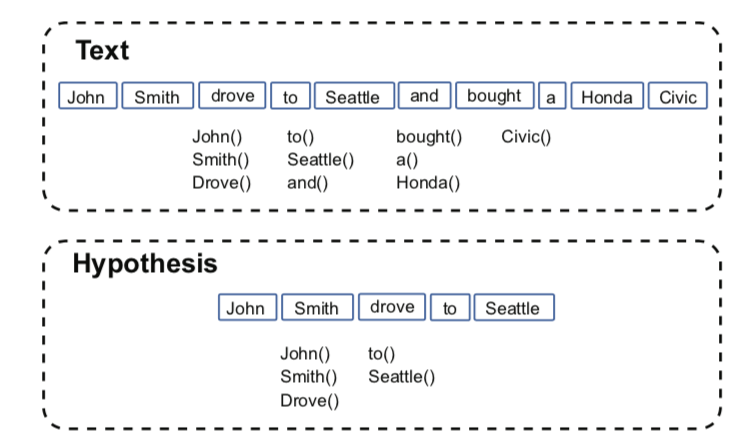
\includegraphics[scale=0.35]{img/lexical_level.png}
}

\frame[<+->]{ \frametitle{Lexical level}
\begin{itemize}
    \item H and T sentences encode aspects of underlying meaning that cannot be captured by the purely lexical representation.
    %\item the word “went” instead of “drove.” A human reader will assign the label TRUE, but lexical model will predict FALSE.
\end{itemize}
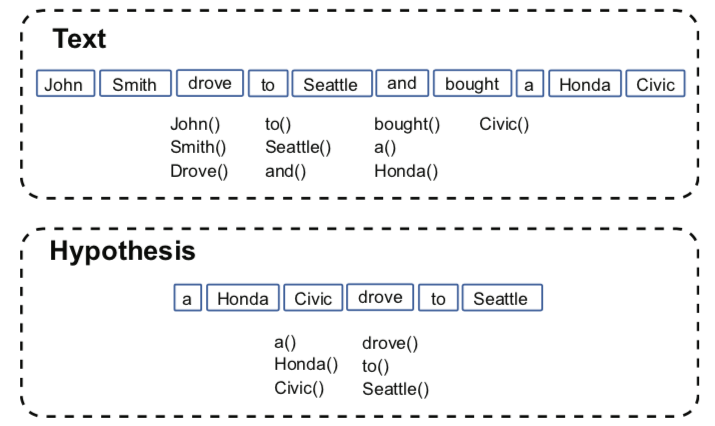
\includegraphics[scale=0.30]{img/lexical_false.png}
}

\frame[<+->]{ \frametitle{Structural level}
\begin{itemize}
    \item Syntactic structure provides cues for the underlying meaning of a sentence. 
   
    
\end{itemize}
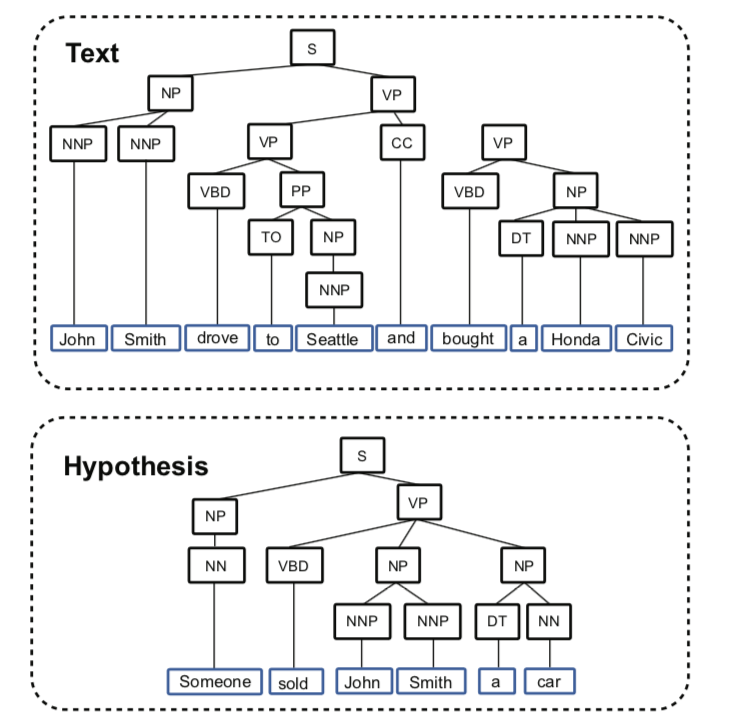
\includegraphics[scale=0.2]{img/struct_level.png}
}


\frame[<+->]{ \frametitle{Structural level}
\begin{itemize}
    \item If T contains the same structure (i.e, dependency edges), the system will predict TRUE and otherwise FALSE. 
    \item  “John” and “drove,” but the two words are \red{separated} by a sequence of dependency edges. 
    \item Given the expressiveness of the dependency representation, many possible sequences of edges that could represent connection, and many other sequences that do not.
\end{itemize}
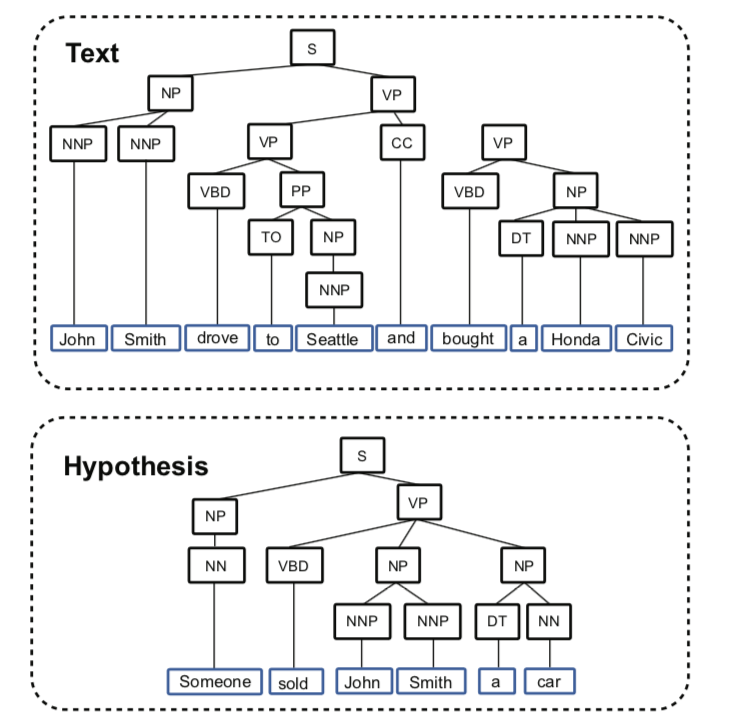
\includegraphics[scale=0.10]{img/struct_level.png}
}

\frame[<+->]{ \frametitle{Semantic level}
\begin{itemize}
    \item Semantic role labelling, grouping of words into “arguments” (entity such as a person or place) and “predicates” (a predicate being a verb representing the state of some entity).
    \item \blue{Immediate connections} between arguments and predicates.
    \item  “John” is an argument of the predicate “drove” 
\end{itemize}
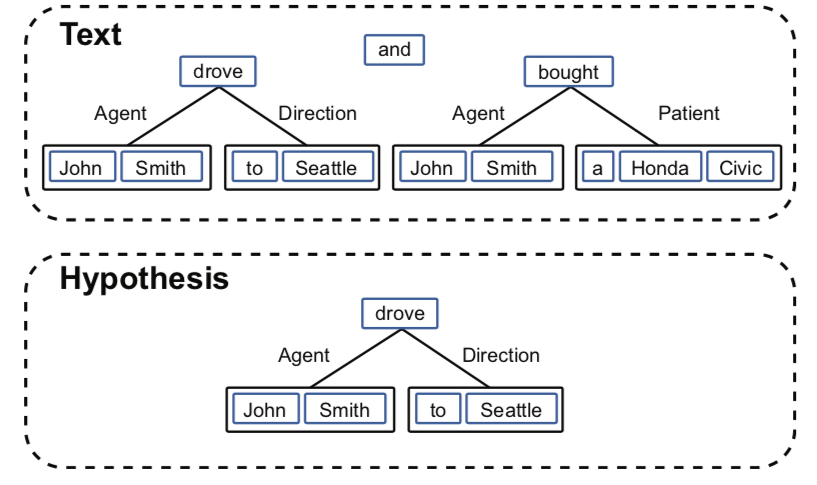
\includegraphics[scale=0.20]{img/semantic_level.png}
}
\frame[<+->]{ \frametitle{Knowledge Acquisition for RTE}
\begin{itemize}
     \item T: The U.S. citizens elected their new president Obama. \\
    H: Obama was born in the U.S.
    \item Assumed \blue{background knowledge}: “U.S. presidents should be naturally born in the U.S.”
\end{itemize}
}

\frame[<+->]{ \frametitle{Knowledge Acquisition for RTE}
\begin{itemize}
   
    \item Knowledge is a lexical-semantic relation between two words.
    \item I enlarged my \blue{stock}. and I enlarged my \blue{inventory}.\\
    \blue{synonym}
    \item I have a \blue{cat}. entails I have a \blue{pet}. \\
    \blue{hyponymy}
    \item But also meaning implication between more complex structures than just lexical terms. \\
    X \textit{causes} Y $\rightarrow$ Y \textit{is a symptom of} X
\end{itemize}
}

\frame[<+->]{ \frametitle{Knowledge Acquisition for RTE}
\begin{itemize}
    \item WordNet specifies \blue{lexical-semantic} relations between lexical items such as hyponymy, synonymy, and derivation. \\
    chair $\rightarrow$ furniture 
    \item FrameNet is a lexicographic resource for \blue{frames} that are events and includes information on the predicates and argument relevant for that specific event.\\
    The attack frame, and specifies events: ‘assailant’, a ‘victim’, a ‘weapon’, etc.\\
    cure X $\rightarrow$ X recover
    \item Wikipedia articles for identifying \blue{is a} relations. \\
    Jim Carrey $\rightarrow$ actor
\end{itemize}
}

\frame[<+->]{ \frametitle{Knowledge Acquisition for RTE}
\begin{itemize}
    \item \textbf{Extended Distributional Hypothesis}: If two paths tend to occur in similar contexts, the meanings of the
paths tend to be similar. 
    \item X solves Y \\
    Y is solved by X \\
X finds a solution to Y
\end{itemize}
}

\frame[<+->]{ \frametitle{Knowledge Acquisition for RTE}
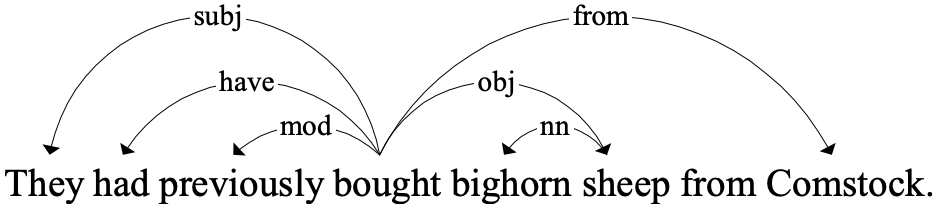
\includegraphics[scale=0.40]{img/deep_dirt.png}\\
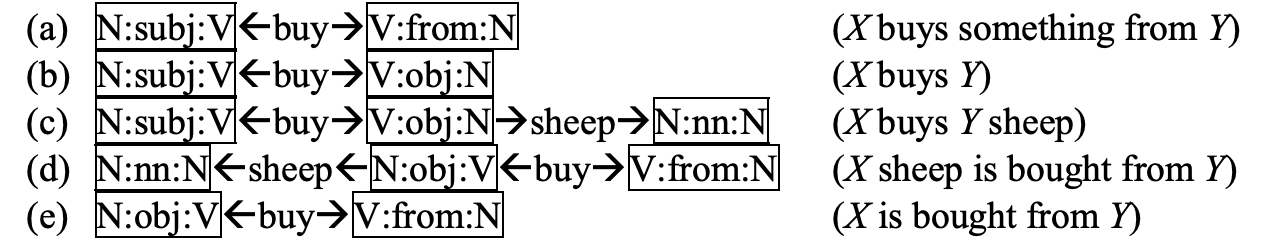
\includegraphics[scale=0.40]{img/rule_dirt.png}
}
 
 

\section{RTE Methods}
\frame[<+->]{ \frametitle{Recognising Textual Entailment Methods}
\begin{itemize}
    \item RTE depend on the representation (e.g. words,
syntax, semantics) of the T-H pair that is used to extract features to train a supervised classifier.
\end{itemize}
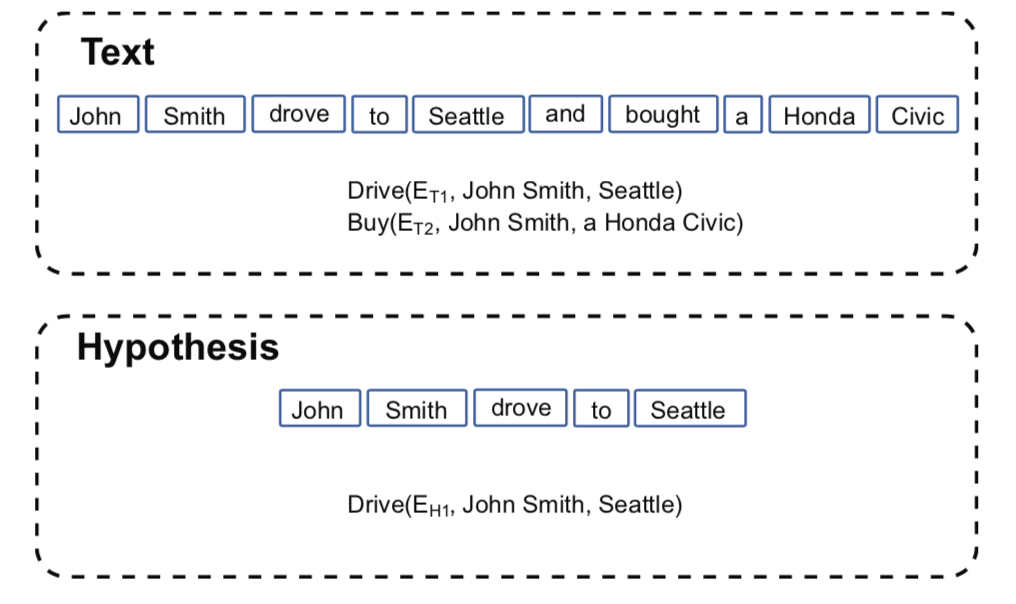
\includegraphics[scale=0.40]{img/meaning_representation.png}
}

\frame[<+->]{ \frametitle{Recognising Textual Entailment Methods}
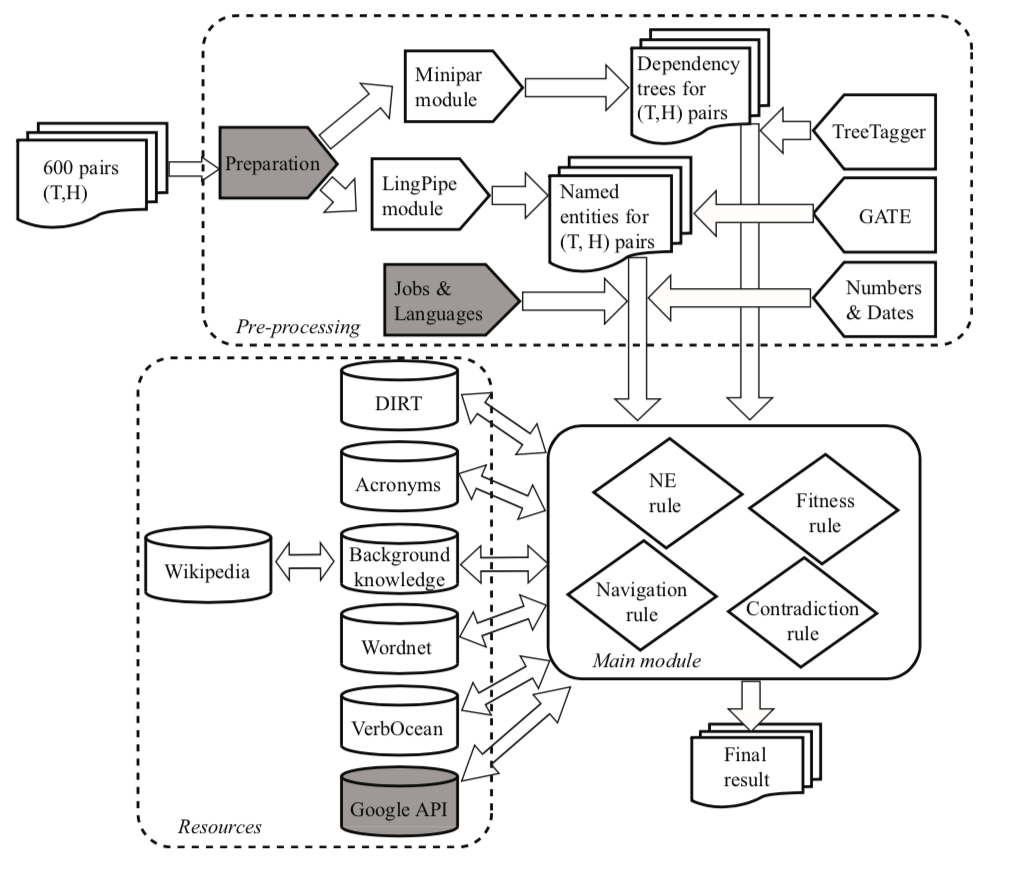
\includegraphics[scale=0.45]{img/rte_system.png}
}

%\subsection{Similarity-based approaches}
\frame[<+->]{ \frametitle{Similarity-based approaches}
\begin{itemize}
\item  Pair with a strong similarity score holds a positive entailment relation. 
    \item Wordnet similarity.
    \item String similarity.
    \item  Similarity scores computed from different linguistic levels. \\ The goal is to find complementary features.
\end{itemize}
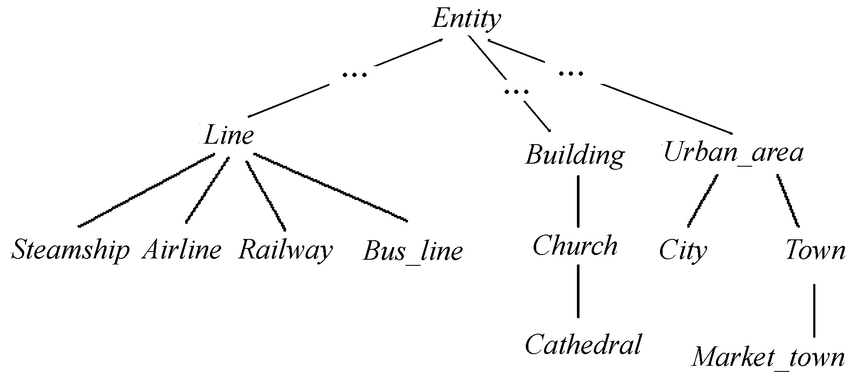
\includegraphics[scale=0.30]{img/Fragment-of-WordNet-concept-taxonomy.png}
}

%\subsection{Alignment-based approaches}
\frame[<+->]{ \frametitle{Alignment-based approaches}
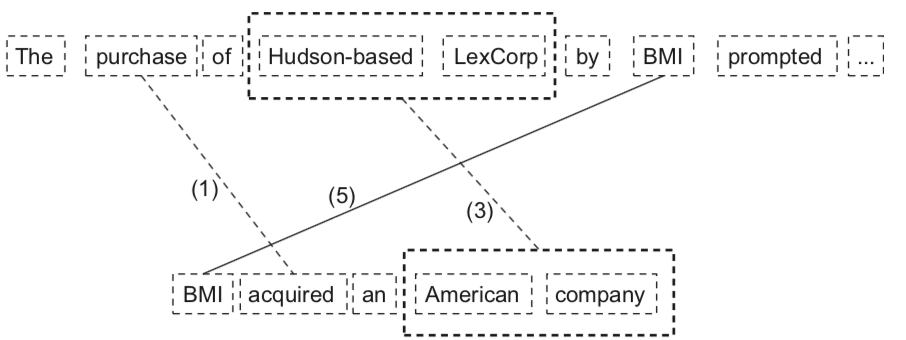
\includegraphics[scale=0.50]{img/alignment.png}
\begin{itemize}
    \item  (1,purchase,acquired) \\
    (3,Hudson-based LexCorp, American company),\\
    (5,BMI,BMI)
\end{itemize}
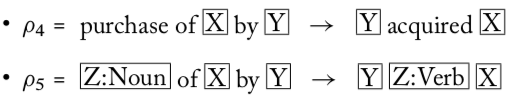
\includegraphics[scale=0.70]{img/alignment_rules.png}
}

\frame[<+->]{ \frametitle{Alignment-based approaches}

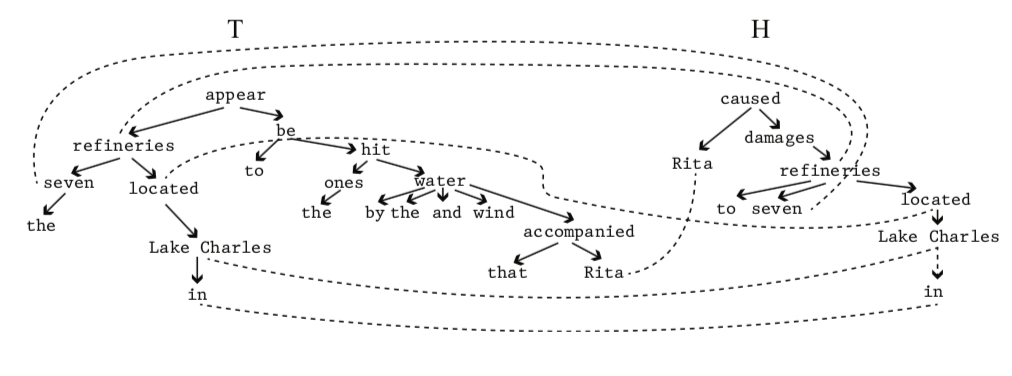
\includegraphics[scale=0.60]{img/deep_alignment.png}


}



%\subsection{Edit distance-based approaches}
\frame[<+->]{ \frametitle{Edit distance-based approaches}
\begin{itemize}
    \item  T entails H if there is a \blue{sequence of transformations} applied to T such that we can obtain H with an overall cost below a certain \blue{threshold}.
    \item Insertion, Substitution, and Deletion.
    \item Alternative for expensive theorem provers.
\end{itemize}
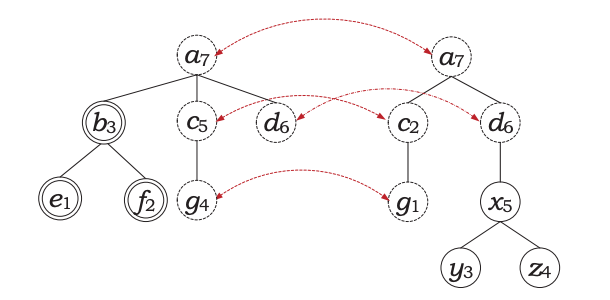
\includegraphics[scale=0.55]{img/TED.png}
}

\subsection{Evaluation}
\frame[<+->]{ \frametitle{Evaluation}
\begin{itemize}
    \item Accuracy 
    \item RTE-3 corpus \red{1,600} T-H pairs\\
    information extraction, information retrieval, question answering, and summarisation. 
    \item  The lexical baseline,  between 55\% and 58\% \blue{accuracy} 
    \item RTE-3 higher scores all system entries suggesting an \red{easier} entailment corpus
    \item RTE-4 and RTE-5 increase the difficulty by adding
 irrelevant signals (additional words, phrases, and sentences).
\end{itemize}
}

\section{Current Methods}




\frame[<+->]{ \frametitle{SNLI}
\begin{itemize}
    \item  Flickr30k corpus for image captioning domaim. \\
    Annotated pairs of texts at sentence level
    \item The relations (i.e. 3-way classification labels) are: \\ \textit{entailment},  \textit{contradiction}, and  \textit{neutral}.
    \item $550,152$ training, $10$K development, and $10$k test.
    \item Premise: A soccer game with multiple males playing. \\
          Hypothesis: Some men are playing a sport.
\end{itemize}
}


\frame[<+->]{ \frametitle{MNLI}
\begin{itemize}
    \item Multiple genres  \\ 
    classifiers only learn \red{regularities} over annotated data, leading to \red{poor generalization} beyond the domain of the training data
    \item \textit{matched} (5 in domain genres) $392,702$ training, \\ $10$k \textit{matched} development, 
    \item $10$k \textit{mismatched} (5 out of domain genres) development. 
    \item T: 8 million in relief in the form of emergency housing. \\
    H: The 8 million dollars for emergency housing was still not enough to solve the problem. \\
    \blue{Government}
\end{itemize}
}




\frame[<+->]{ \frametitle{Drawbacks}

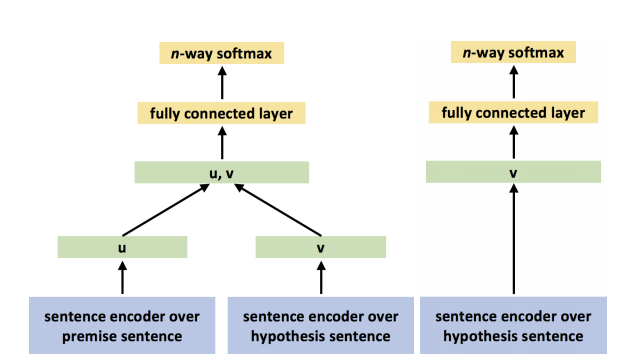
\includegraphics[scale=0.45]{img/hyp_only.png} \\
%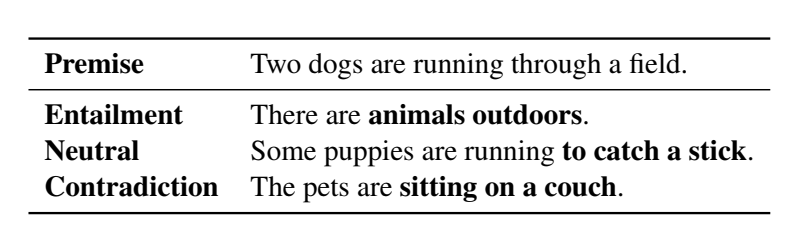
\includegraphics[scale=0.50]{img/snli-artifacts1.png}\\
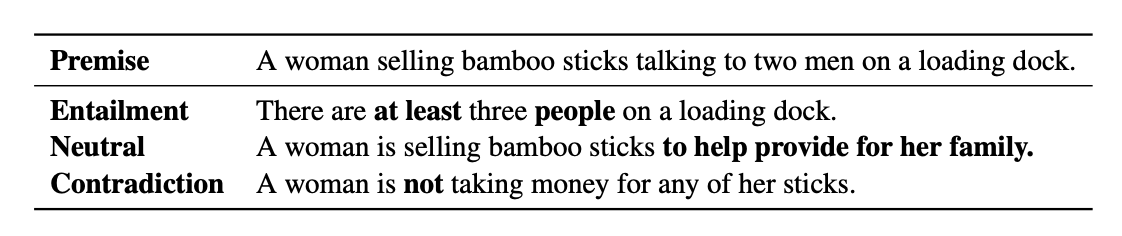
\includegraphics[scale=0.45]{img/snli-artifacts2.png}
\begin{itemize}
    \item Entailment: animal, instrument, and outdoors.
    \item Neutral: Modifiers (tall, sad, popular) and superlatives
(first, favorite, most)
    \item Contradiction: Negation words, nobody, no, never and nothing
\end{itemize}
\ack{\citep{glockner-etal-2018-breaking}}
}




\frame[<+->]{ \frametitle{Neural Network Models}
\begin{itemize}
    \item Embeddings like glove or elmo, for fine tuning.
    \item Sentence representations.
\end{itemize}]
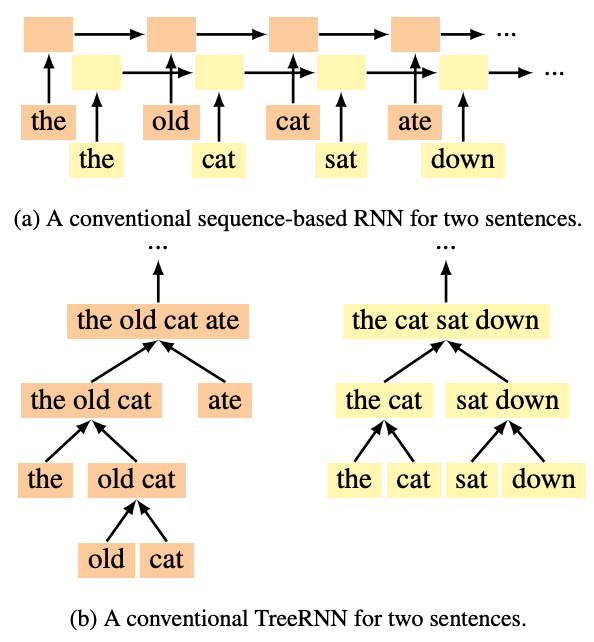
\includegraphics[scale=0.40]{img/tree-lstm_composition.png}
}

\frame[<+->]{ \frametitle{BiLSMT composition}
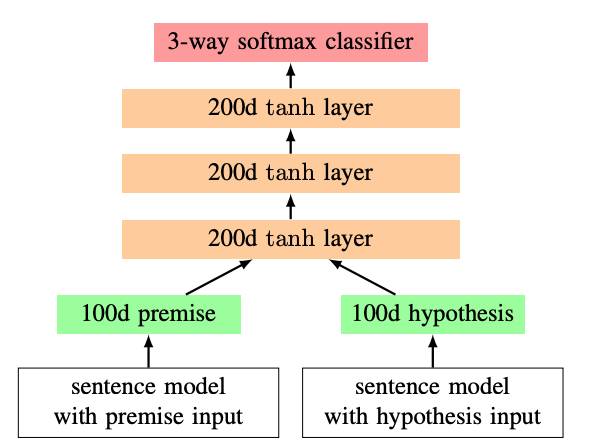
\includegraphics[scale=0.60]{img/lstm_model.png}
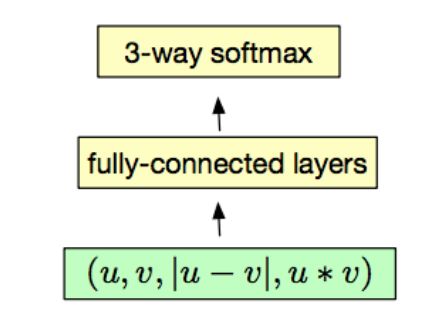
\includegraphics[scale=0.30]{img/sum_composition.png}
%\todo{add mix of features interaction}
}


\frame[<+->]{ \frametitle{ESIM}
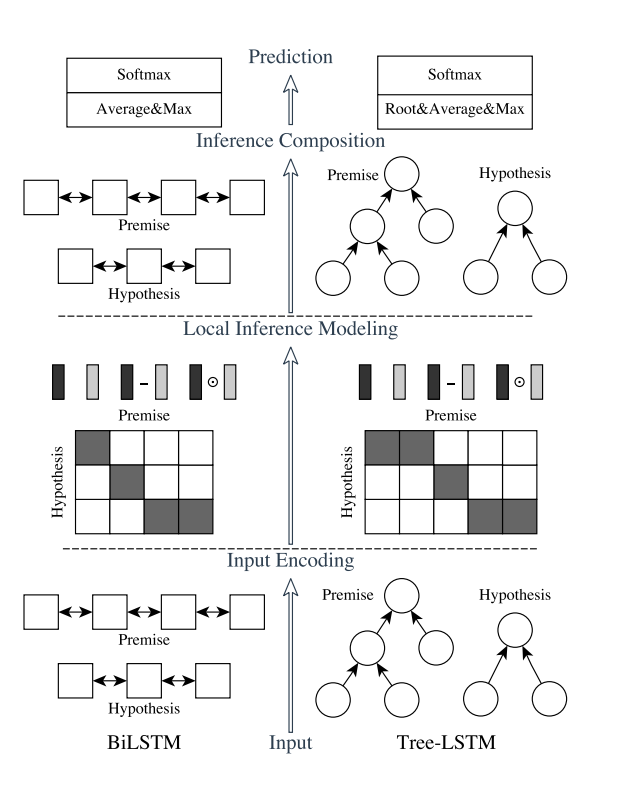
\includegraphics[scale=0.53]{img/esim.png}
\ack{\citep{chen2017enhanced}}
}

\frame[<+->]{ \frametitle{ESIM}
\scriptsize{
\begin{subequations}
\begin{align}
    \mathbf t_i &= \emb(t_i; \omega_{\text{emb}}) \\
    \mathbf h_j &= \emb(h_j; \omega_{\text{emb}}) \\
    \mathbf s_1^m &= \birnn(\mathbf t_1^m; \omega_{\text{enc}})  \\
    \mathbf u_1^n &= \birnn(\mathbf h_1^n; \omega_{\text{enc}})  \\
   \mathbf a_i &= \att(\mathbf s_i, \mathbf u_1^n)  \\
    \mathbf b_j &= \att(\mathbf u_j, \mathbf s_1^m)  \\
    \mathbf c_i &= [\mathbf s_i, \mathbf a_i, \mathbf s_i - \mathbf a_i, \mathbf s_i \odot \mathbf a_i] \\
    \mathbf d_j &= [\mathbf u_j, \mathbf b_j, \mathbf u_j - \mathbf b_j, \mathbf u_j \odot \mathbf b_j] \\
    \mathbf c_1^m &= \birnn(\mathbf c_1^m; \omega_{\text{comp}}) \\
    \mathbf d_1^n &= \birnn(\mathbf d_1^n; \omega_{\text{comp}}) \\
    \mathbf q &= [\avg(\mathbf c_1^m), \maxpool(\mathbf c_1^m),  \avg(\mathbf d_1^n), \maxpool(\mathbf d_1^n)] \\
    \mathbf q &= \tanh(\affine(\mathbf q; \omega_{\text{hid}})) \\
    f(x) &= \softmax(\mlp(\mathbf q; \omega_{\text{cls}})) 
\end{align}
\end{subequations}
}
}

%\frame[<+->]{ \frametitle{Neural Network Models}
%}

\section{Latent Variable Models}

\frame[<+->]{ \frametitle{Latent Structure Induction}
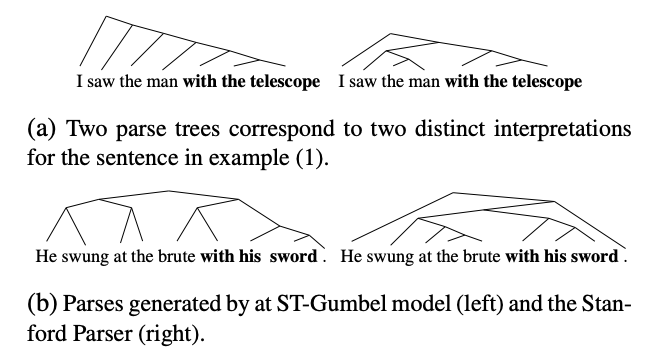
\includegraphics[scale=0.60]{img/gumbel-spinn_trees.png}\\
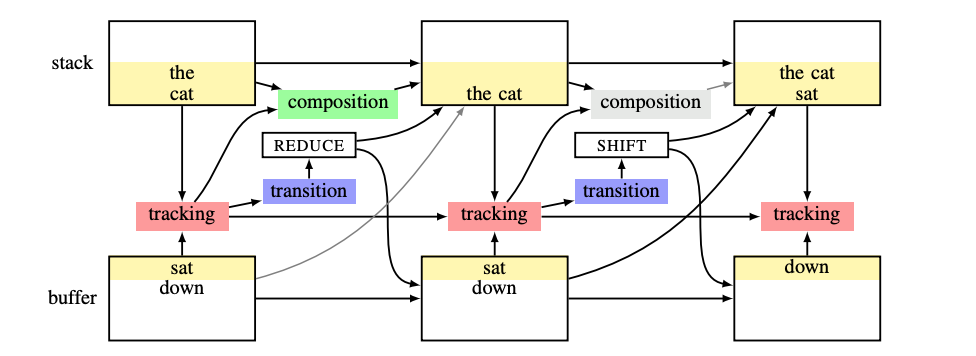
\includegraphics[scale=0.30]{img/spinn.png}
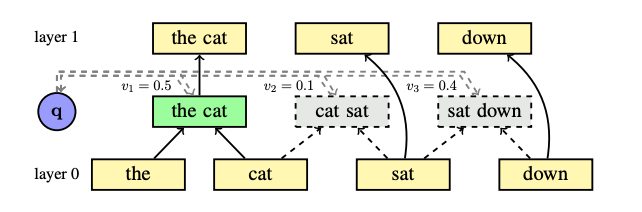
\includegraphics[scale=0.50]{img/gumbel.png}
}

\frame[<+->]{ \frametitle{Deep Generative Models}
\begin{itemize}
    \item Model that generates \blue{hypothesis} and \blue{decision} given a text and a stochastic embedding of the hypothesis-decision pair.
    \item Models to learn from mixed-domain NLI data \\ e.g. by capitalising on lexical domain-dependent patterns. 
    \item Performance of standard classifiers tend to vary across domains and especially out of domain.
\end{itemize}
%
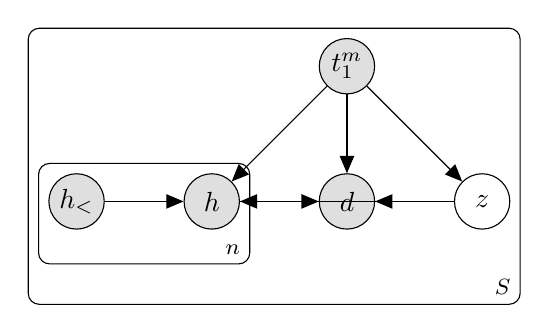
\begin{tikzpicture}

\node[obs]		(t_g)		{$ t_1^m $};
\node[obs, below = of t_g]		(d_g)		{$ d $};
\node[latent, right = of d_g]						(z_g)		{$ z $};
\node[obs, left = of d_g]		(h_g)		{$ h $};
\node[obs, left = of h_g]		(h_g_past)		{$ h_{<} $};
%\node[below = of d_g]           (theta)      {$ \theta $};

\edge{t_g}{z_g,d_g};
\edge{t_g}{h_g};
\edge{h_g_past}{h_g};
\edge{z_g}{d_g}
\edge[bend left]{z_g}{h_g};
\edge{h_g}{d_g};
%\edge{theta}{d_g,h_g,z_g}

% add plates
%\plate {text} {(t_g)}{$ m $} 
\plate {hypo} {(h_g) (h_g_past)}{$ n $}
\plate {corpus} { (t_g) (z_g) (d_g) (hypo)} {$ S $};  %  (text)
\end{tikzpicture}

\begin{align*}
 Z_i| t_1^m &\sim \mathcal N(\mu(s_1^m), \sigma^2(s_1^m)) \\ %& i \in \{1, \ldots, m\} \\
H_i|z_1^m &\sim Cat(f(z_1^m, t_1^m; \theta)) \\ %& i \in \{1, \ldots, m\} \\
D_j|z_1^m, h_1^n  &\sim Cat(g(z_1^m, t_1^m, h_1^n; \theta))  %& i \in \{1, \ldots, d\} 
\end{align*}

}

\frame[<+->]{ \frametitle{Deep Generative Models}

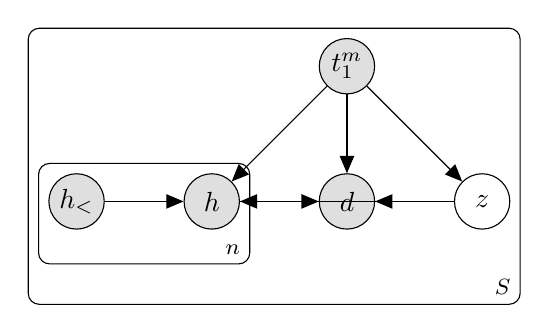
\begin{tikzpicture}

\node[obs]		(t_g)		{$ t_1^m $};
\node[obs, below = of t_g]		(d_g)		{$ d $};
\node[latent, right = of d_g]						(z_g)		{$ z $};
\node[obs, left = of d_g]		(h_g)		{$ h $};
\node[obs, left = of h_g]		(h_g_past)		{$ h_{<} $};
%\node[below = of d_g]           (theta)      {$ \theta $};

\edge{t_g}{z_g,d_g};
\edge{t_g}{h_g};
\edge{h_g_past}{h_g};
\edge{z_g}{d_g}
\edge[bend left]{z_g}{h_g};
\edge{h_g}{d_g};
%\edge{theta}{d_g,h_g,z_g}

% add plates
%\plate {text} {(t_g)}{$ m $} 
\plate {hypo} {(h_g) (h_g_past)}{$ n $}
\plate {corpus} { (t_g) (z_g) (d_g) (hypo)} {$ S $};  %  (text)
\end{tikzpicture}

\begin{align*}
 Z_i| t_1^m &\sim \mathcal N(\mu(s_1^m), \sigma^2(s_1^m)) \\ %& i \in \{1, \ldots, m\} \\
H_i|z_1^m &\sim Cat(f(z_1^m, t_1^m; \theta)) \\ %& i \in \{1, \ldots, m\} \\
D_j|z_1^m, h_1^n  &\sim Cat(g(z_1^m, t_1^m, h_1^n; \theta))  %& i \in \{1, \ldots, d\} 
\end{align*}

}

\frame[allowframebreaks]{ \frametitle{Deep Generative Models}
\footnotesize{
\begin{itemize}
\item Joint likelihood of y (hypothesis) and d (decision) \\
\begin{equation}
\begin{aligned}
    p(y,d|x, \theta) = \\
    \int p(z|x, \theta)p(y|x,z, \theta)p(d|x,y,z, \theta) d z .
\end{aligned}
\end{equation}
\item The \emph{hypothesis generation model}: \\ 
\begin{equation}
    \begin{aligned}
        &p(y|x,z, \theta) = \prod_{j=1}^{|y|} p(y_j|x, z, y_{<j}, \theta) \\
        &= \prod_{j=1}^{|y|} \Cat(y_j|f_o(x, z, y_{<j}; \theta)) ~ ,
    \end{aligned}
\end{equation}
\item The \emph{classification model} ESIM:\\
\begin{equation}
    p(d|x, y, z, \theta) = \Cat(d|f_c(x, y, z; \theta)) 
\end{equation}
\item Lowerbound on the log-likelihood function  (ELBO) \\
\begin{equation}
    \begin{aligned}
        \mathcal L(\theta, \phi) = \mathbb E_{q(z|x, y, d, \phi)}\left[  \log p(y, d|x, z, \theta)\right] \\
        - \KL(q(z|x, y, d, \phi)||p(z|x, \theta))
    \end{aligned}
\end{equation}
\end{itemize}
}
}

\frame[<+->]{\frametitle{Deep Generative Models}
\begin{tabular}{lcc}
\toprule
Model                & \multicolumn{2}{c}{Dev}                  \\ 
\multicolumn{1}{l}{} & \multicolumn{1}{c}{matched}  & mismatched\\ \midrule
%BiLSTM               &            67.86                 &      67.31      &       &                                \\
%BiLSTM-VAE           &             69.00                &     68.70       &       &                                \\ 
ESIM$_\text{mnli}$                 &          $74.39\pm0.11$                   &  $74.05\pm0.21$           \\


~ + $\mathcal{N}$-VAE$_\text{50z}$            &             $74.89\pm0.25$          &     $74.07\pm0.37$        \\
~ + $\mathcal{N}$-VAE$_\text{100z}$            &             $74.82\pm0.28$          &      $73.91\pm0.59$        \\
~ + $\mathcal{N}$-VAE$_\text{256z}$            &              $74.87\pm0.15$         &      $74.08\pm0.16$        \\
%\quad - disentanglement             &                $74.47\pm0.13$            &    $73.88\pm0.55$     \\ 

%\midrule
%~ + $\mathcal{S}$-VAE$_\text{10z,1.0k}$            &             $74.82\pm0.11$           &      $74.59\pm0.02$        \\
\bottomrule
\end{tabular}

}

\section{Uncertainty in Natural Language Inference}


%\frame[<+->]{ \frametitle{Uncertainty in natural language inference}
%\begin{itemize}
%\item MOTIVATION

%\item MC Dropout
%\item VI RNN
%\end{itemize}

%}

\frame[<+->]{ \frametitle{Bayes by backprop}
\begin{itemize}
\item NNs perform well with lots of data, however they fail to express uncertainty with little or no data, \\
 leading to overconfident decisions.
 \item Bayesian neural networks introduce probability distributions over the weights. 
\end{itemize}
\begin{figure}
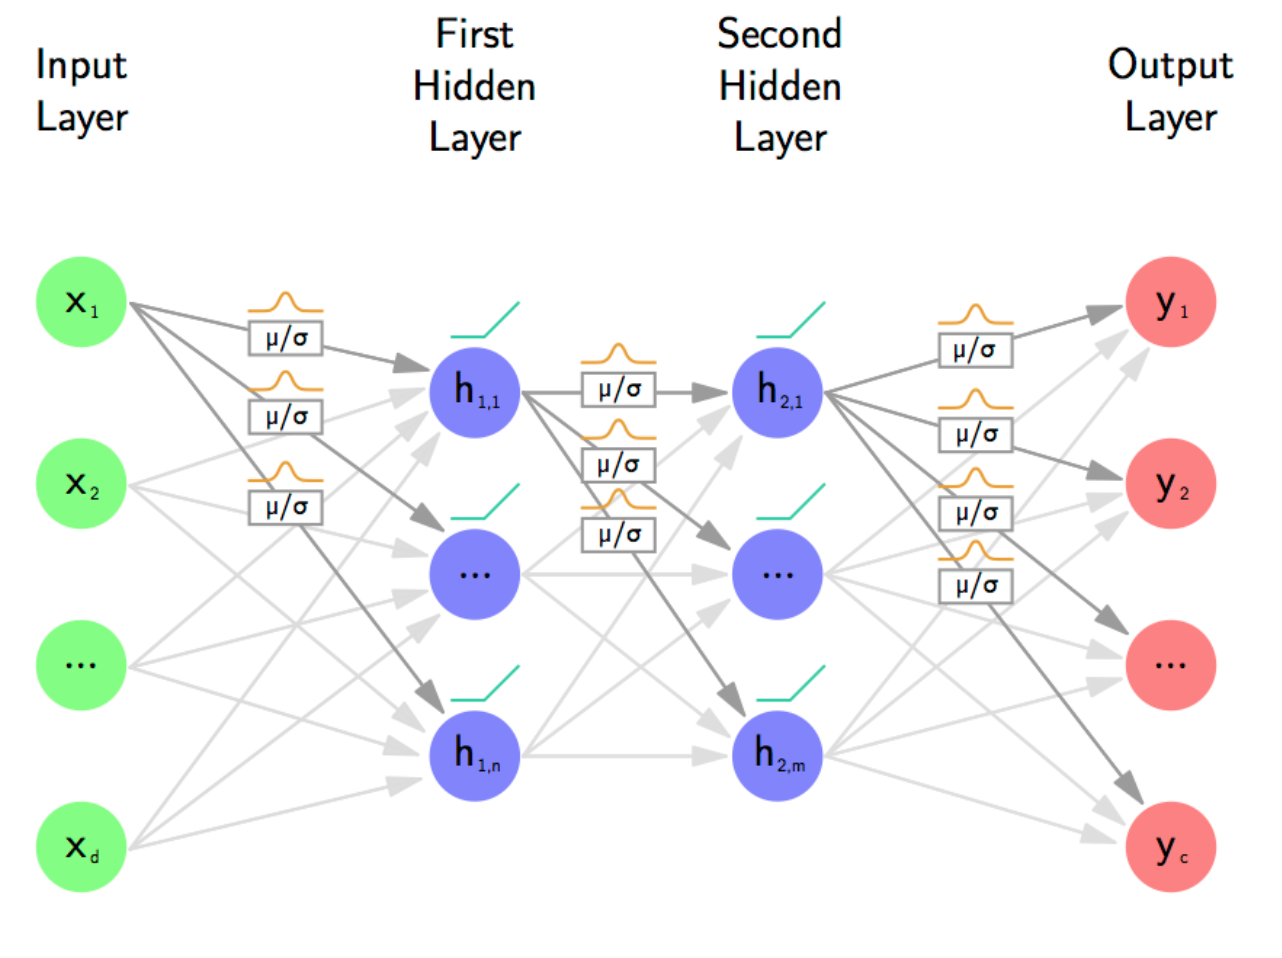
\includegraphics[scale=0.2]{img/bnn}
\end{figure}
}


\frame[<+->]{ \frametitle{Bayes by backprop}
\footnotesize{
\begin{itemize}
\item However, Bayesian inference on the parameters $\omega$ of a neural network is intractable, with data $D$. 
\begin{equation}
p(\omega | \mathcal{D})=\frac{p(\mathcal{D} | \omega) p(\omega)}{p(\mathcal{D})} =\frac{p(\mathcal{D} | \omega) p(\omega)}{\int p(\mathcal{D} | \omega) p(\omega) \mathrm{d} \omega}
\end{equation}
\item We need an approximation $q(\omega | \theta)$, over the weights that approximates the true posterior
\item The ELBO is:\\
\begin{equation}
\begin{aligned} 
\mathcal{L}(\mathcal{D}, \theta) &=\int q(\omega | \theta) \log \frac{q(\omega | \theta)}{p(\omega)}-q(\omega | \theta) \log p(\mathcal{D} | \omega) \mathrm{d} \omega \\ &=\mathrm{KL}[q(\omega | \theta) \| p(\omega)]-\mathbb{E}_{q(\omega | \theta)}[\log p(\mathcal{D} | \omega)] \end{aligned}
\end{equation}
\end{itemize}
}
\ack{\citep{Blundell:2015:WUN:3045118.3045290}}
}

%\subsection{Deep Generative Models}

\frame[allowframebreaks]{\frametitle{MC dropout}
\begin{itemize}
\item On NLI training inputs $X = \langle (t_1, h_1), \ldots, (t_n, h_n)  \rangle$ are premise ($t$) and hypothesis ($h$) pairs, and the corresponding outputs $Y = \langle y_1, \ldots, y_n \rangle$ over $N$ instances. 
\item The likelihood for classification is defined by: \\
\begin{equation}
\begin{aligned}
    p(y|x, \omega ) = \Cat(y|f(x; \omega)) ,
\end{aligned}
\end{equation} \\
over $y$ entailment relations computed by mapping from the input to the class probabilities with a neural network $f$ parameterised by $\omega$. 
\item  A Bayesian NN \citep{MacKay:1992:PBF:148147.148165} is defined by placing a prior distribution over the model parameters $p(\omega)$, where this prior is often a Gaussian distribution $p(\omega) \sim \mathcal N (0, I)$.
\item  The Bayesian NN formulation leads to a posterior distribution over the parameters given our observed data, instead of a single estimate.  
\item We are interested on estimating the posterior distribution over the parameters  $p(\omega | \mathcal{D})$, given our observed data $X, Y$.
\item  The goal is to predict a new input instances by marginalising over the parameters: \\

\begin{equation}
\begin{aligned}
    p(y^*|x^*, \mathcal{D}) =  \int p(y^*|x^*, \omega)p(\omega|\mathcal{D}) d \omega  .
\end{aligned} 
\end{equation}

\item However, the true posterior $p(\omega | \mathcal{D})$ is intractable, and \citet{doprout_gal16} use variational inference  to approximate this posterior. 

\item We define an approximate distribution $q_\theta(\omega)$, to minimise the $\KL$ divergence between the approximation and the true posterior. 

\item The objective for optimisation is  a lower-bound  on  the  log-likelihood function (ELBO): \\
\begin{equation}
\begin{aligned}
    \mathcal L =  \mathbb E_{q(\omega)} \left[\sum_{i=1}^{N} \log p(y_i | f(x_i; \omega))\right]\\ -\KL(q_{\theta}(\omega))||p(\omega)), 
\end{aligned}
\label{objective}
\end{equation} \\
where the $\KL$ term is approximated with $L_2$ regularisation.
\item  \citet{doprout_gal16} show that the use of dropout  in NNs before each weight layer is an approximation to variational inference in Bayesian NNs.

%Dropout is a common regularisation technique  for NNs.
%\item \citet{virnnGal} extend the variational dropout to RNNs to define a variational RNN. The variational RNN dropout repeats the same mask at each time step for inputs, outputs, and states. 

\item By replacing the true posterior $p(\omega| \mathcal{D})$ with the approximate posterior $q_\theta(\omega)$, we obtain a Monte Carlo (MC) estimate for future predictions : \\
\begin{equation}
\begin{aligned}
    p(y^*|x^*, \mathcal{D}) &\approx  \int p(y^*|x^*, \omega)q_\theta(\omega) d \omega \\
    &\approx \frac{1}{T}\sum_{t}^{T}p(y^{*}|x^{*}, \hat{\omega}_t),
\end{aligned}
\end{equation} \\
where $\hat{\omega}_t \sim q_\theta(\omega)$%Moreover, sampling from $q(\omega)$ is similar to applying dropout on a NN layer. 
\item In practice, the approximation to the predictive distribution is based on performing $T$ stochastic forward passes through the network and averaging the results.
\item  In other words, this is achieved by performing \blue{dropout at test time} (MC dropout).
\item Finally, for classification, a way to quantify uncertainty is by computing the entropy of the output probability vector $\mathcal H(p) = - \sum_{c=1}^{C} p_c \log p_c$ over $c$ classes.




\end{itemize}

}

\frame[<+->]{ \frametitle{Uncertainty in natural language inference}
\begin{itemize}
\item ESIM for classification  (without syntactic parses)
\item The word embedding and the bidirectional LSTMs are shared between the pair of texts. A single ($\tanh$) hidden layer MLP with a $\softmax$ output predicts the class probabilities.
\item We use dropout on both the LSTM (variational RNN), and the word embedding. 
\item In the word embedding $\omega_{ \text{emb}} \in \R^{V \times D}$, with $V$ vocabulary and $D$ dimensionality, the dropout masks types (rows) instead of words in a sequence .
\item Finally, for the additional $L_2$ regularisation, we use a separate weight decay: for weights $\lambda_{\omega} = \frac{1 - p_{\text{drop}}}{ N }$ with $p_{\text{drop}}$ dropout, and for biases ($b$): $\lambda_{\text{b}} =  \frac{1}{ N}$.
\end{itemize}

}


\frame{\frametitle{Results}
\begin{tabular}{clcc}
\toprule
 Training                      & Model  & SNLI & Breaking NLI \\ \midrule
%\multirow{2}{*}{*ESIM}
\multirow{3}{*}{SNLI} & ESIM$^\dagger$ &  87.9  &  65.6 \\
\cmidrule{2-4}
                      & ESIM$_\text{ours}$ & $86.4\pm0.09$ &      $57.6\pm1.9$ \\
                      & ESIM$_\text{MC}$ & $86.5\pm0.13$ &  $68.9\pm1.7$ \\
\midrule
\multirow{3}{*}{MNLI+SNLI} & ESIM$^\dagger$ & 86.3  &    74.9 \\
\cmidrule{2-4}
                      & ESIM$_\text{ours}$ & $86.8\pm0.05$  &     $68.8\pm3.5$ \\
                      & ESIM$_\text{MC}$ & $86.6\pm0.16$ &  $75.2\pm1.3$  \\
 
\bottomrule
\end{tabular}
}


\frame{\frametitle{Results SNLI}
\begin{figure}
   
    \subfloat{{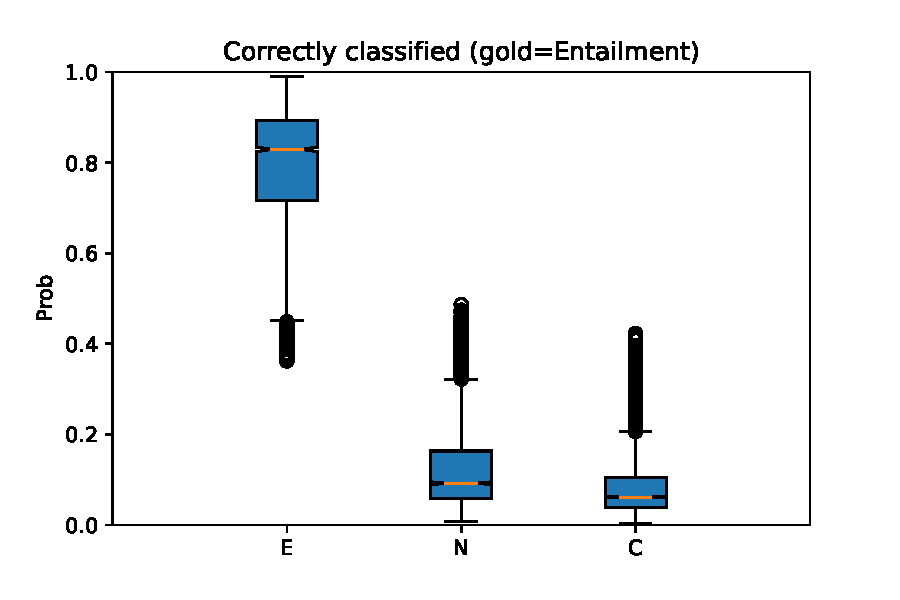
\includegraphics[scale=0.2]{img/snli-testSnli-gEcorrect_bplot.pdf} }}%
    ~ 
    \subfloat{{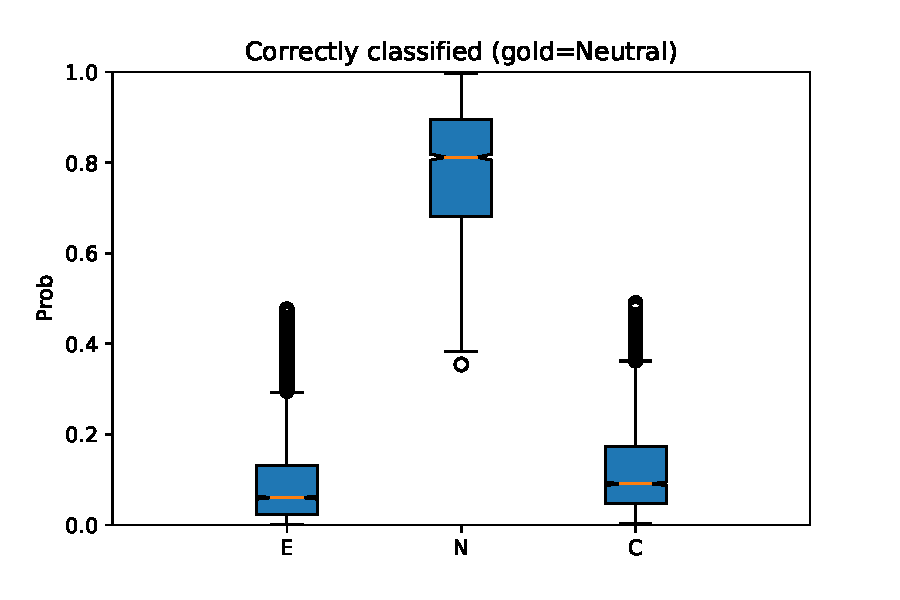
\includegraphics[scale=0.2]{img/snli-testSnli-gNcorrect_bplot.pdf} }}%
   ~
    \subfloat{{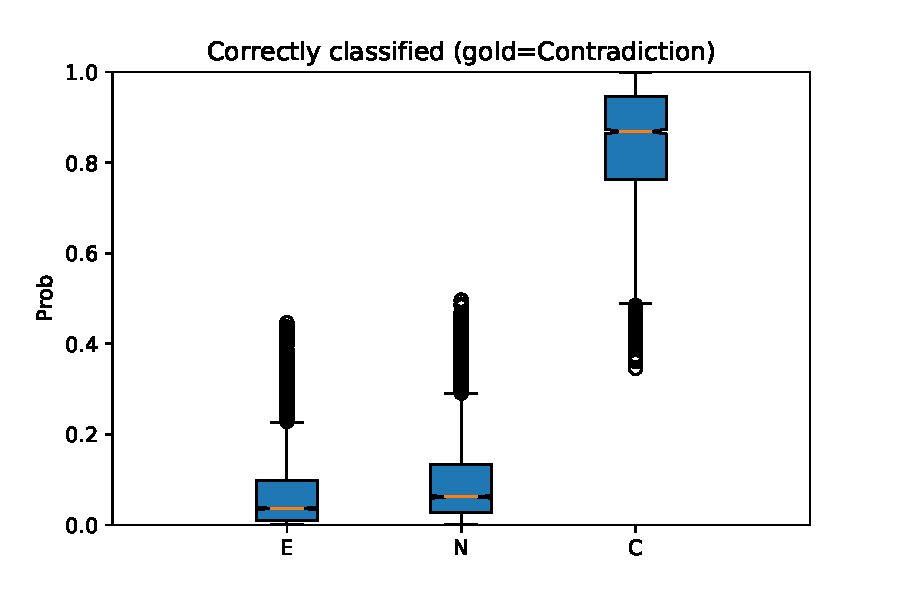
\includegraphics[scale=0.2]{img/snli-testSnli-gCcorrect_bplot.pdf} }}%
 

\end{figure}  

 \begin{figure}
    
    \subfloat[Gold label entailment.]{{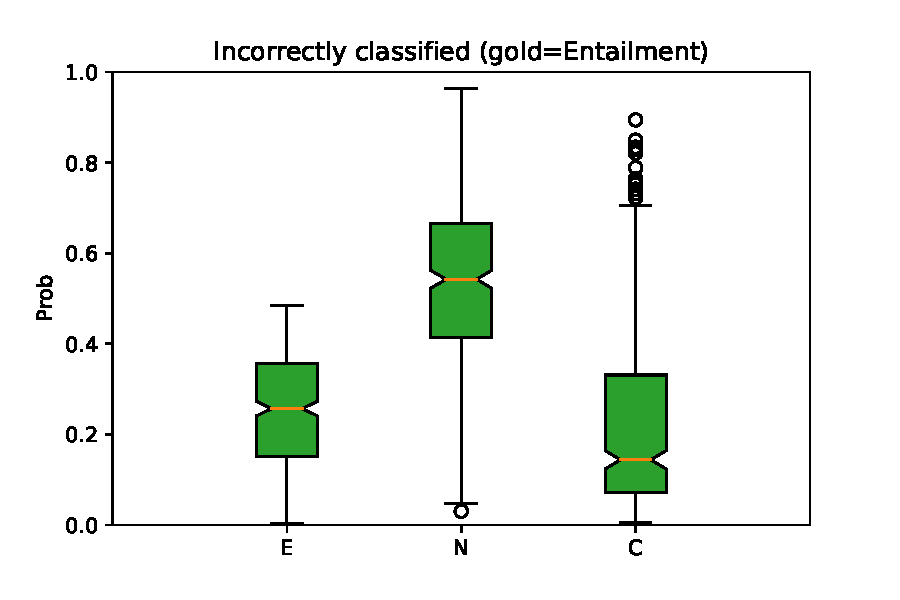
\includegraphics[scale=0.2]{img/snli-testSnli-gEincorrect_bplot.pdf} }}
    ~
    \subfloat[Gold label neutral.]{{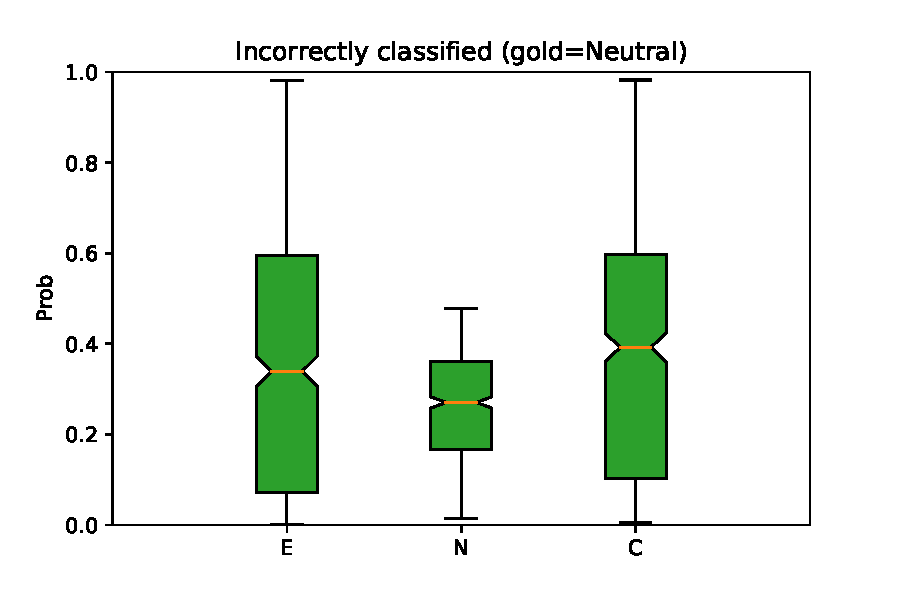
\includegraphics[scale=0.2]{img/snli-testSnli-gNincorrect_bplot.pdf} }}
    ~
    \subfloat[Gold label contradiction.]{{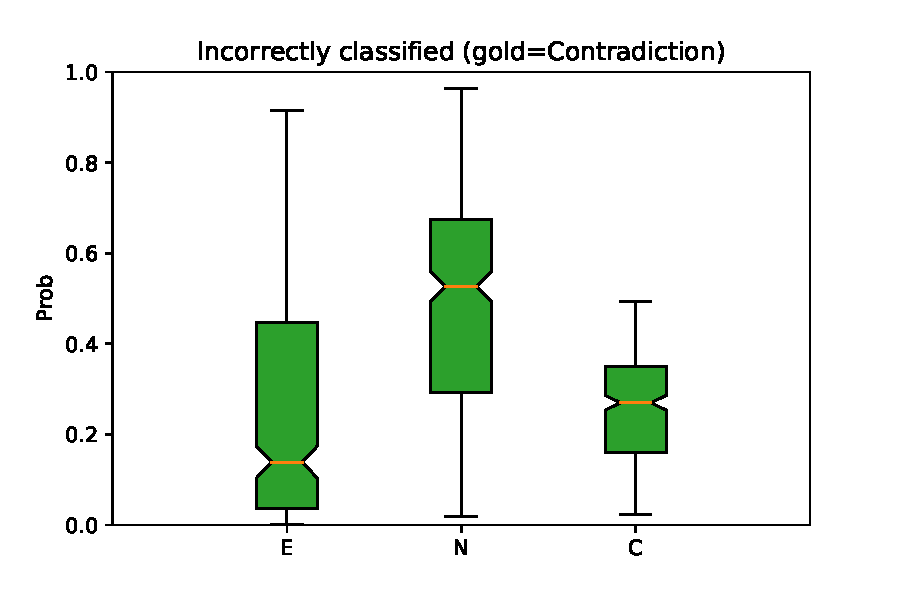
\includegraphics[scale=0.2]{img/snli-testSnli-gCincorrect_bplot.pdf} }}
   
\end{figure}
}



\frame{\frametitle{Results SNLI and Breaking}
 \begin{figure}%

    \subfloat[SNLI]{{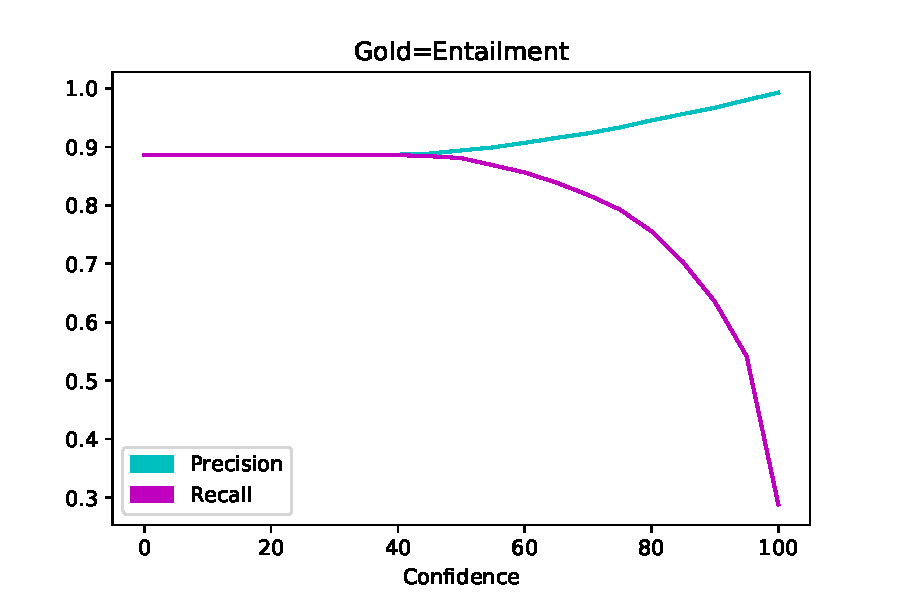
\includegraphics[scale=0.20]{img/snli0_pvr.pdf} }}%
    ~ 
    \subfloat{{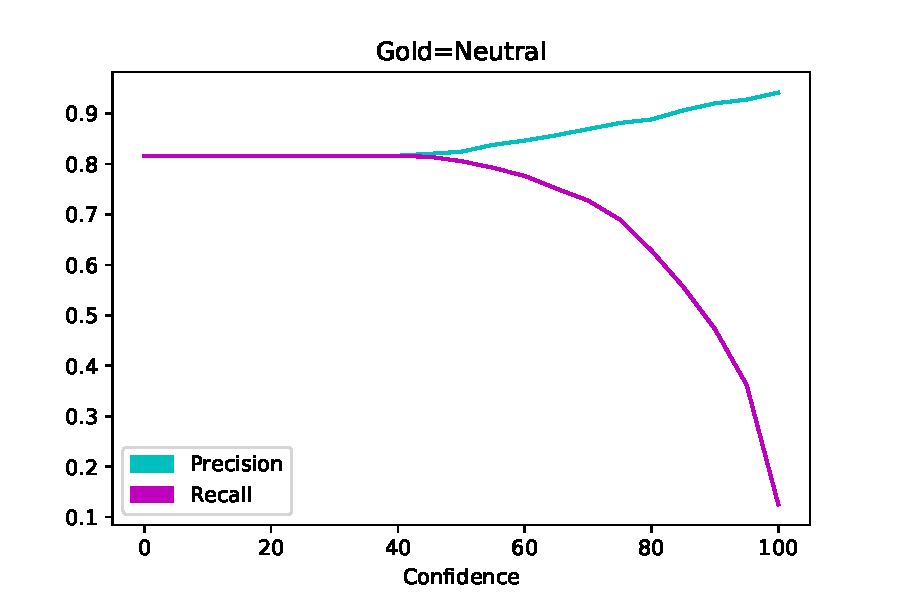
\includegraphics[scale=0.2]{img/snli1_pvr.pdf} }}%
   ~
    \subfloat{{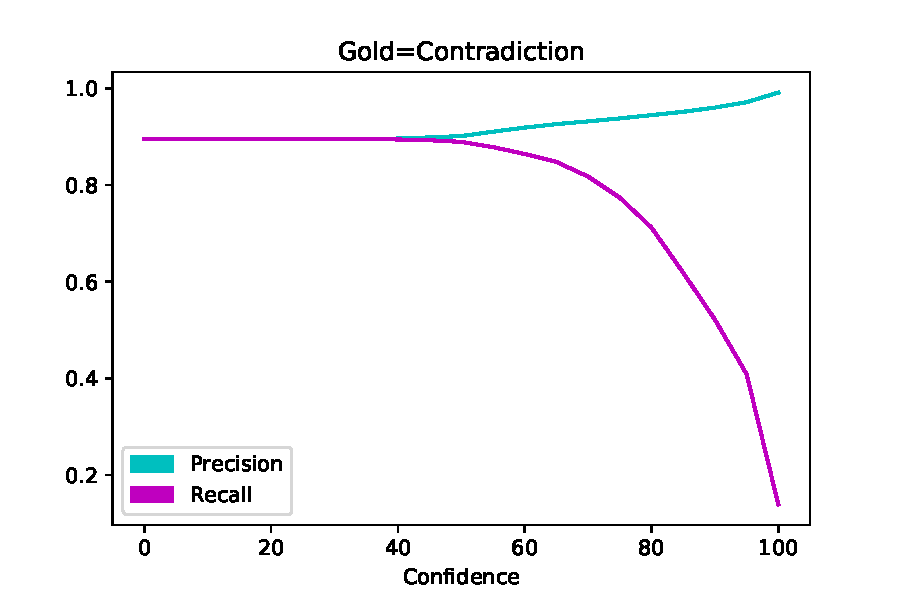
\includegraphics[scale=0.2]{img/snli2_pvr.pdf} }}%

   % \caption{Precision and recall for different confidence thresholds on SNLI.}%
 
\end{figure}  

 \begin{figure}%

    \subfloat[Breaking]{{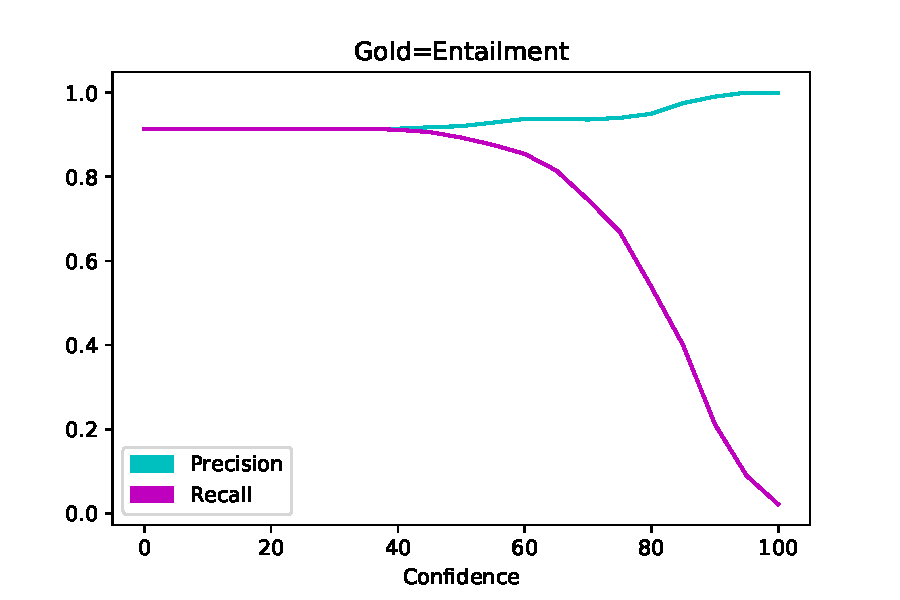
\includegraphics[scale=0.2]{img/breaking0_pvr.pdf} }}%
    ~ 
    \subfloat{{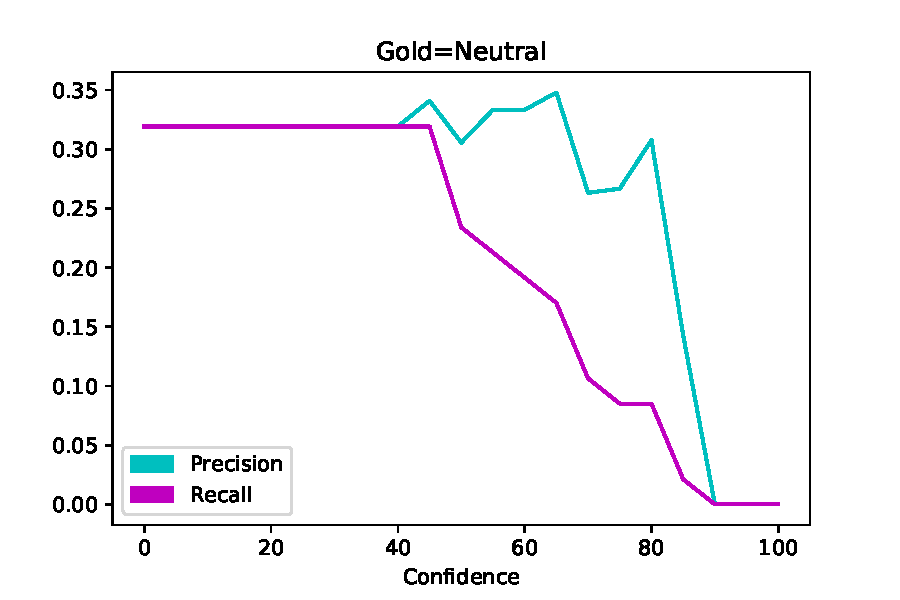
\includegraphics[scale=0.2]{img/breaking1_pvr.pdf} }}%
   ~
    \subfloat{{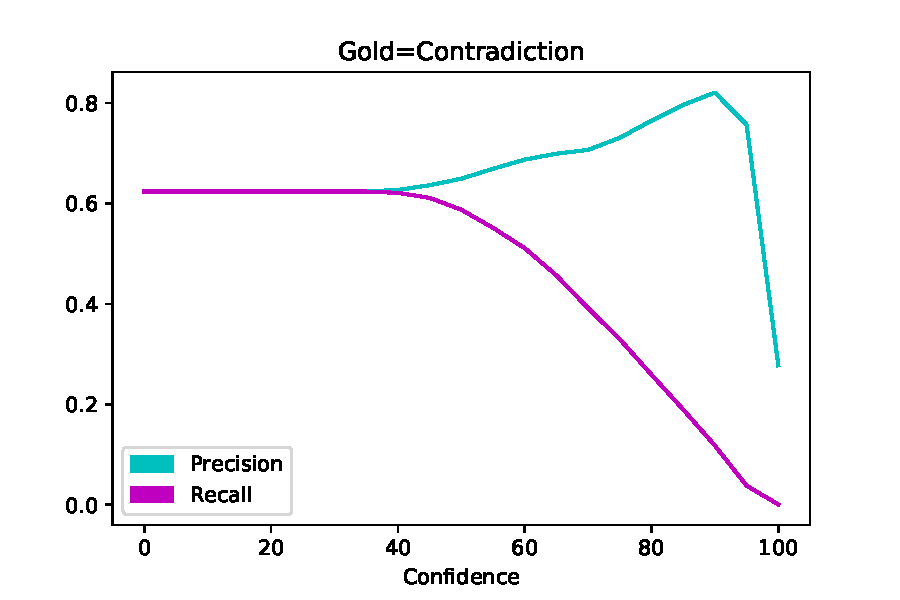
\includegraphics[scale=0.2]{img/breaking2_pvr.pdf} }}%

    %\caption{Precision and recall for  different confidence thresholds on Breaking NLI.}%
    %\label{fig:precreacBreak}%
\end{figure}
}




%\frame{\frametitle{Results}

%}



\frame{\frametitle{Results}

   \begin{tabular}{cl}  
         \begin{tabular}{c}
           
            \parbox{0.27\linewidth}{%  change the parbox width as appropiate
            \begin{tiny}
            P: The {\color{blue}little} girl is riding in the car with her dad. \\
            H: The {\color{blue}small} girl is riding in the car with her dad. \\
           
            P: The little girl is riding in the car with her {\color{red}dad}. \\
            H: The little girl is riding in the car with her {\color{red}father}. \\
           
            P: The {\color{applegreen}little} girl is riding in the car with her dad. \\
            H: The {\color{applegreen}tiny} girl is riding in the car with her dad. \\
            \end{tiny}
    }
           \end{tabular}
           & \begin{tabular}{l}
            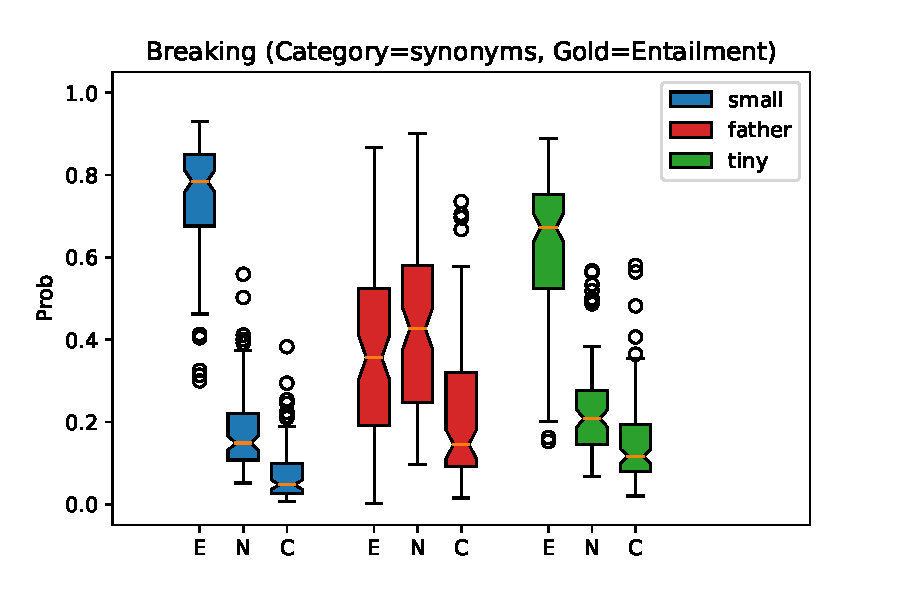
\includegraphics[width=5.5cm]{img/eg_breaking_16395-16397.pdf}
         \end{tabular} \\
\end{tabular} 

}

\frame{\frametitle{Homework!!}
\begin{itemize}
\item Dropout in Recurrent Networks \citep{gal2016theoretically}
\item Use the same dropout mask at each time step for both inputs, outputs, and recurrent layers
\item The RNN can be framed as a probabilistic model.
\end{itemize}
\begin{figure}
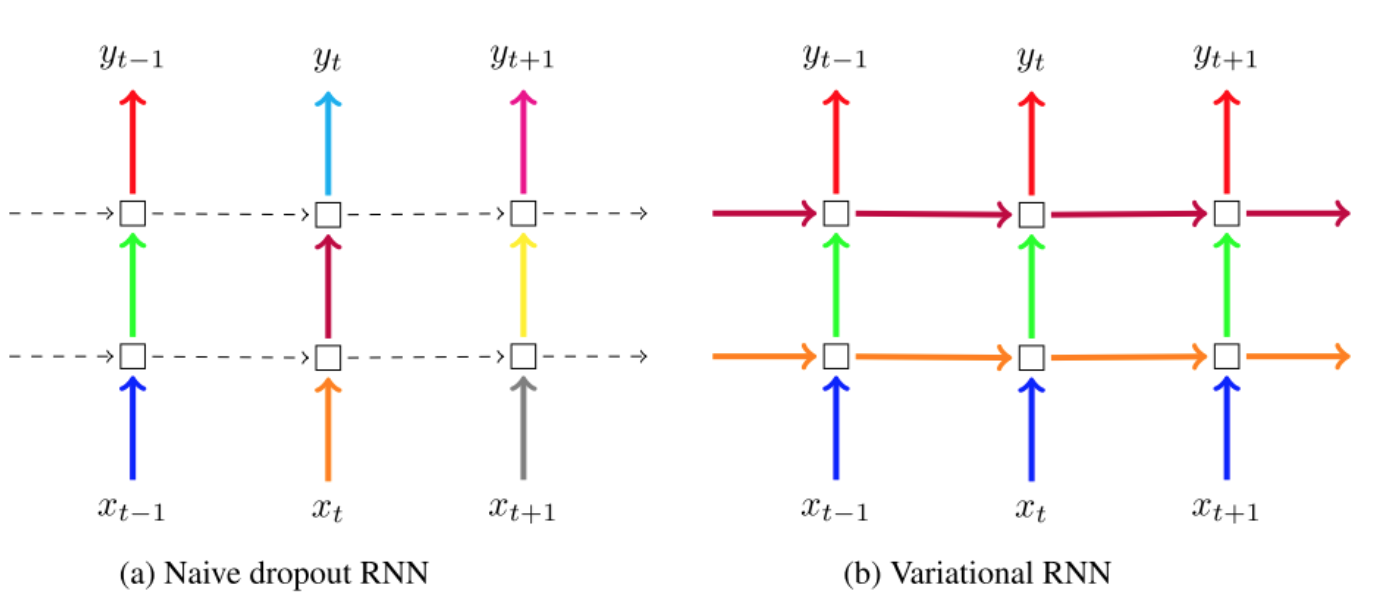
\includegraphics[scale=0.35]{img/viRNN}
\end{figure}
}


\begin{frame}[allowframebreaks]{Literature}
\bibliographystyle{plainnat}
\small
\bibliography{BIB}
\end{frame}


\end{document}
\grid
